
\section{Performance Analysis}
\label{sec:performance-analysis}

In this section, we discuss the performance of \sahad{} in terms of the overall work
and time complexity.
Throughout this section, we denote the
number of nodes and edges in the network by $n$ and $m$ respectively. We use $k$
to represent the number of nodes in the template. 

%We also analyze the time complexity of the
%intermediate stage -- a stage between the Mapper and Reducer -- that always
%behaves as a bottle neck for the overall performance.



\iffalse
\begin{lemma}
\label{lemma:colorer}

The sizes of the input and output of the Algorithm~\ref{alg:colorer-mapper} are
both $O(|E_G|)$.

\end{lemma}

\begin{proof}

	The input to the \textit{Mapper} consists of $(v,N(v))$ for $\forall v \in
	V_G$, where the size of $N(v)$ equals $d(v)$.
Therefore, the size of the input is $O(|E_G|)$.  Similarly, the size of the
output is also $O(|E_G|)$, since it consists of $v,X_{T_0,v},N(v)$ for $\forall
v \in V_G$.

\end{proof}
\fi

%\noindent
%\textbf{Work Complexity.} 

\begin{lemma}
\label{lemma:counter}
For a template $T_i$, suppose the sizes of the two sub-templates $T_i'$ and
$T_i''$ are $k_i'$ and $k_i''$, respectively, the sizes of the input, output, and
work complexity corresponding to a node $v$ are given below:

\begin{itemize}

\item The sizes of the input and output of Algorithm~\ref{alg:counter-mapper}
 are $O({k \choose k_i'} + {k \choose k_i''} + d(v))$ and $O({k \choose
 k_i''}d(v))$, respectively.

\item The size of the input to Algorithm \ref{alg:counter-reducer} is $O({k \choose k_i''}d(v))$.
%, and its work complexity is $O({k \choose k_i'} {k \choose k_i''}d(v))$.

\end{itemize}

\end{lemma}

\begin{proof} 

For a node $v$, the input to Algorithm~\ref{alg:counter-mapper} involves the
corresponding $X_{T_i',v}$ and $X_{T_i'',v}$ for $T_i'$ and $T_i''$, as well as
$N(v)$, which together have size $O({k \choose k_i'} + {k \choose k_i''} +
d(v))$.  If the input is for $T_i''$, Algorithm \ref{alg:counter-mapper}
generates multiple key-value pairs for a node $v$, in which each key-value pair
corresponds to some node $u \in N(v)$.  Therefore, the output has size $O({k
\choose k_i''}d(v))$.

For a given $v$, the input to Algorithm \ref{alg:counter-reducer} is the
combination of the above, and therefore, has size $O({k \choose k_i''}d(v))$. 
\hfill\ensuremath{\blacksquare}
\end{proof}

\begin{lemma}
\label{lemma:workcomp}
The total work complexity is $O(k|E_G|2^{2k}e^k\log{(1/\delta)}\frac{1}{\varepsilon^2})$.
\end{lemma}
\begin{proof}

For node $v$ and each neighbor $u \in N(v)$, Algorithm \ref{alg:counter-reducer}
aggregates every pair of the form $(S_a,C_a)$ in $X_{T_i',v}$, and $(S_b,C_b)$
in $X_{T_i'',u}$, which leads to a work complexity of $O({k \choose k_i'} {k \choose k_i''}d(v))$.
%For each node $v$ and template $T_i
%\in\mathcal{T}$, the work complexity of Algorithm \ref{alg:counter-reducer} is $O({k \choose
%k_i'}{k \choose k_i''}d(v))$. 
Since $|\mathcal{T}|\leq k$, the total work, over all nodes and templates is at most

\begin{equation}
\hspace*{-0.2in}O(\sum_{v, T_i} {k \choose k_i'} {k \choose k_i''} d(v)) = O(\sum_vk2^{2k}d(v)) = O(k|E_G|2^{2k})
\end{equation}

Since $O(e^k\log{(1/\delta)}\frac{1}{\varepsilon^2})$ iterations are performed
in order to get the $(\varepsilon,\delta)$-approximation, the lemma follows.
\hfill\ensuremath{\blacksquare}
\end{proof}


\noindent
\textbf{Time Complexity.}
We use $P$ to denote the number of machines. We assume each machine is configured to run
a maximum of $M$ Mappers and $R$ Reducers simultaneously.
%and each of the Mappers takes a block of the data
%with $B$ entries. We also use $R$ to denote the number of Reducers running on
%each machine simultaneously. 
Finally, we assume a uniform partitioning, so that each machine processes $n/P$ nodes.

%With a uniform partitioning as the original setting used for
%\sahad{}, i.e., each partition has the same number of nodes $n/P$, that
%will be processed by a machine. 

\begin{lemma}
\label{lemma:colorer-counter-mapper}
The time complexity of Algorithm~\ref{alg:colorer-mapper} and 
\ref{alg:counter-mapper} is $O(\frac{n}{PM})$ and $O(\frac{m}{PM})$, respectively.

\end{lemma}

\begin{proof}

We first consider Algorithm~\ref{alg:colorer-mapper}, which takes as input an
entry of the form $(v, N(v))$ for some node $v$, and perform a constant work.
There are $\frac{n}{P}$ entries processed by each machine. Since $M$ Mappers are
run simultaneously, this gives a running time of $O(\frac{n}{PM})$.  Next, we
consider Algorithm~\ref{alg:counter-mapper}. Each Mapper outputs $(v, X)$ for
input $T'_i$ and $d$ entries for input $T''_i$ for each $u \in N(v)$, where $d$
is the degree of $v$. Therefore, each computing node performs
$O(\sum_{i=1}^{n/P}{d_i})=O(m/P)$ steps. Here $d_i$ is the degree for $v_i$.
Again, since $M$ Mappers run simultaneously, the total running time is $
O(\frac{m}{PM})$.

\hfill\ensuremath{\blacksquare}
\end{proof}
%In Algorithm~\ref{alg:colorer-mapper}, each input entry $(v, N(v))$ represents a
%node $v$ and its neighbors. Since each Mapper processes $B$ entries, the running
%time of a Mapper is $O(B)$.  The number of Mappers on a machine to process
%$\frac{n}{P}$ entries is $\frac{n}{PB}$. So the serialized running time is
%$\frac{n}{PB} \cdot O(B) = O(\frac{n}{P})$. Since we can simulteously run $M$
%Mappers, the running time of Algorithm~\ref{alg:colorer-mapper} is
%$O(\frac{n}{PM})$. 
%
%In Algorithm~\ref{alg:counter-mapper}, each Mapper output one entry $(v, X)$ for
%$T'_i$ and $d$ entries for $T''_i$ for $\forall u \in N(v)$. Here $d$ is the
%degree of $v$. So the running time of a Mapper is $O(dB)$. Given that the number
%of Mappers is $O(\frac{n}{PB})$ as denoted in last paragraph, the serialized
%running time is $O(\frac{n}{PB}) \cdot O(dB) = O(\frac{nd}{P})$. Given $M$
%Mappers are running simutaneously, the running time of Algorithm
%~\ref{alg:counter-mapper} is $O(\frac{nd}{PM}) = O(\frac{m}{PM})$.

%TODO \textcolor{red}{parallel algorithm may not reduce running time linearly, revise}


\begin{lemma}
\label{lemma:counter-reducer}
The time complexity of Algorithm~\ref{alg:counter-reducer} is $O(\frac{m \cdot 2^{2k}}{PR})$.
\end{lemma}
\begin{proof}
Suppose $|S'_i| = k'_i$ and $|S''_i| = k''_i$. The number of possible
color sets $S'_i$ and $S''_i$ is $k \choose k'_i$ and $k \choose k''_i$,
respectively. Line 2 of Algorithm~\ref{alg:counter-reducer} involves $O({k \choose
k'_i}) = O(2^k)$ steps.  Similarly, line 4 also involves $O(2^k)$ steps and
Line 3 involves $O(d)$ steps.
Therefore the totally running time is $O(d) \cdot 2^{2k}$.
Each machine processes $\frac{n}{P}$ entries corresponding to different nodes,
leading to a total of $O(\frac{nd \cdot 2^{2k}}{P})$ steps. Since $R$ reducers
run in parallel on each machine, this leads to a total time of $O(\frac{m \cdot 2^{2k}}{PR})$.
%TODO \textcolor{red}{parallel algorithm may not reduce running time linearly, revise}
\hfill\ensuremath{\blacksquare}
\end{proof}

\begin{lemma}
\label{lemma:sum}
The time complexity of Algorithm~\ref{alg:sum-mapper} and \ref{alg:sum-reducer}
is $O(\frac{n}{PM})$ and $O(n)$, respectively.
\end{lemma}
\begin{proof}
Algorithm~\ref{alg:sum-mapper} maps out a single entry for each input. Following the
same outline as the proof of~\ref{lemma:colorer-counter-mapper}, its running time is
$O(\frac{n}{PM})$.  Algorithm~\ref{alg:sum-reducer} will take $O(n)$ time since
we have only one key ``sum'', and only one Reducer will be assigned for the
summation for all $v \in V(G)$, which takes $O(n)$ time. 
\hfill\ensuremath{\blacksquare}
\end{proof}

\begin{lemma}
\label{lemma:total}
The overall running time of \sahad{} is bounded by %by Eq.~\ref{eq:total-time}. 
\begin{equation}
\label{eq:total-time}
\begin{array}{lcl}
O(\frac{k2^{2k}m}{P} \cdot (\frac{1}{M}+\frac{1}{R})e^k\log{(1/\delta)}\frac{1}{\varepsilon^2})
%O(k \cdot \frac{m}{P} \cdot \frac{2^{2k}}{R}e^k\log{(1/\delta)}\frac{1}{\varepsilon^2})
\end{array}
\end{equation}
\end{lemma}
\begin{proof}
Algorithm~\ref{alg:colorer-mapper} takes $O(\frac{n}{PM})$ time. Algorithm
~\ref{alg:counter-mapper} and \ref{alg:counter-reducer} run for each step of the
dynamic programming, i.e., joining two sub-templates into a larger template as
shown in Figure~\ref{fig:example-dp}. Since the number of total sub-template is
$O(k)$ when $T$ is a tree, Algorithm~\ref{alg:counter-mapper} and
~\ref{alg:counter-reducer} run $O(k)$ times. Therefore the total time is 
$O(k \cdot (\frac{m}{PM} + \frac{m \cdot 2^{2k}}{PR})) = 
O(\frac{k2^{2k}m}{P} \cdot (\frac{1}{M}+\frac{1}{R})$.
%O(k \cdot \frac{m}{P} \cdot \frac{2^{2k}}{R}).
Finally, the entire algorithm as to be repeated
$O(e^k\log{(1/\delta)}\frac{1}{\varepsilon^2})$ times,
in order to get the $(\varepsilon,\delta)$-approximation, and the lemma follows.
\hfill\ensuremath{\blacksquare}
\end{proof}



\subsection{Performance Analysis of Intermediate Stage}

With \sahad{}, a major bottleneck of a hadoop job in terms of running time
is the shuffling and sorting cost in the intermediate stage between Mapper and
Reducer, due to the high I/O and synchronization cost as shown by the black bar
in Figure~\ref{fig:sahad-breakdown}.

\begin{figure}[htbp]
\centerline{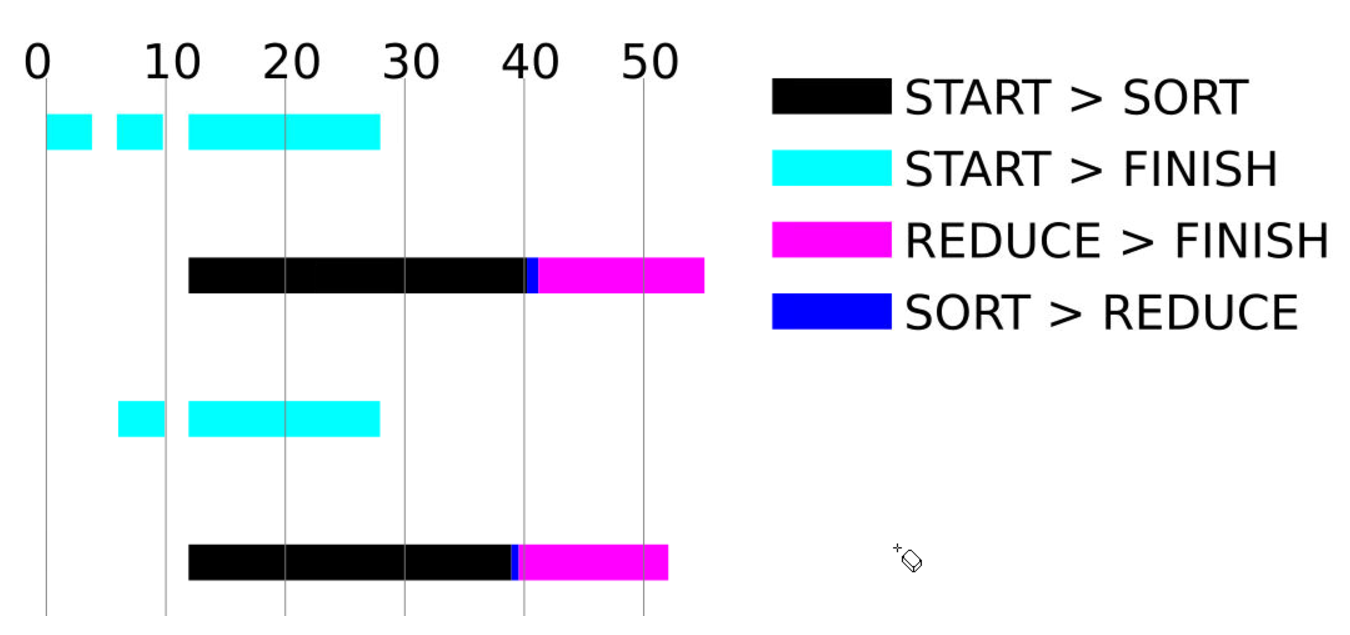
\includegraphics[width=0.30\textwidth]{plots/sahad-breakdown.eps}}

\caption{The figure shows the time spent in each stage of a running hadoop job
to produce count for a 5-node template, by aggregating the 2-node and 3-node
sub-tree. The black bar is the time for intermediate stage, which is for
shuffling and sorting.} 

\label{fig:sahad-breakdown} 
\end{figure}

\iffalse
In \sahad{}, the job running Algorithm~\ref{alg:counter-mapper} and
~\ref{alg:counter-reducer} is mostly computationally intensive among the jobs
that runs other algorithms. We hereby give the running time of its intermediate
stage in lemma~\ref{lemma:intermediate}. 

\begin{lemma}
\label{lemma:intermediate}

Suppose the single message passing operation among two machines takes time $i$,
and the total number of outgoing edges among partitions is $|E_{out}|$, the
cost of the intermediate stage between the mapper (Algorithm
~\ref{alg:counter-mapper}) and Reducer (Algorithm \ref{alg:counter-reducer})
tasks is $O(\frac{m}{P} \log {\frac{m}{P})} + |E_{out}| \cdot i)$.

\end{lemma}

\begin{proof}

Suppose we partition $G$ evenly, then each partition contains $\frac{n}{P}$
nodes. In Algorithm~\ref{alg:counter-mapper}, the total number of entries
produced by mapper on each machine is $\frac{(d+1)n}{P}$. Therefore, the
internal sorting takes $O(\frac{(d+1)n}{P} \cdot \log{\frac{(d+1)n}{P}})$.
After the sorting is completed, each Reducer begins to copy the results it
needs, from both local machine and peers. Suppose $v_1$ and $v_2$ are neighbors
and locate in partition $P_1$ and $P_2$, respectively, then the Reducer
handling $v_2$ needs to copy the entry produced by the mapper which handles
$v_1$, i.e., the entry needs to be delivered from the machine storing $P_1$ to
the machine storing $P_2$. Obviously, the number of entries delivered among
machines equals the total number of edges among partitions. 

\end{proof}

\fi

we observe that the external shuffling and sorting stage takes roughly twice the
time of the reducing stage in Reducers, which dramatically
increase the overall running time. Given that the keys in Mappers and Reducers are
always the index of all the node $v \in V(G)$, we can enhance \sahad{} by
removing the shuffling and sorting in the intermediate stage. Instead, we can
designate Reducers and directly send the data to corresponding Reducers. 

\iffalse
From Lemma~\ref{lemma:intermediate}, we observe that a major performance
bottleneck for our parallel algorithm is induced by two terms: the intermediate
sorting, i.e., $O(\frac{m}{P} \log {\frac{m}{P}})$, and the
communication cost among computing nodes, i.e., $E_{out} \cdot i$. In the
following we will investigate how to reduce the cost brought by these two
terms. And we will examine in the experiment section the effect of optimizing
towards the two factors.
\fi



